\documentclass[12 pt]{amsart}

\usepackage{amssymb}
\usepackage{latexsym}
\usepackage{graphicx}
\usepackage{verbatim}
\usepackage{enumerate}
\usepackage{amsmath}
\usepackage{fullpage}

\begin{document}
\graphicspath{{/home/noah/Documents/MATH\_115\_Number\_Theory/}}

\allowdisplaybreaks
\title
[Problem Set 5]
{Problem Set 5 \\
MATH 115 \\
Number Theory \\
Professor Paul Vojta}

\author{Noah Ruderman}

\date{ July 28, 2014}

\maketitle
\begin{center}
	Problems 3.2.7, 3.2.8, 3.2.18, 3.3.4, 3.3.15, 3.4.1a-f, 3.3.4, 3.3.10, 3.5.1, 3.5.3, 3.5.11, and 3.5.12 
	from \emph{An Introduction to The Theory of Numbers}, 
	$5^{\text{th}}$ edition,
	by Ivan Niven, Herbert S. Zuckerman, and Hugh L. Montgomery 
\end{center}

% PROBLEM 1
\newpage
\phantom{\quad} \vfill
\noindent
\textbf{Problem} (3.2.7) \\[4ex]
\emph{Solution.} \\[2ex]
  We aim to find for which primes $p$ the congruence
  $x^2 \equiv 13 \mod p$
  has a solution.

  First we note that $p = 2$ and $p = 13$ are trivial 
  solutions because both congruence classes of 2 are 
  quadratic residues and $0^2 \equiv 0 \mod 13$.
  Next we note that the congruence will have a solution if the 
  Legendre symbol
  $\left( \frac{13}{p} \right)$
  is equal to 1, by definition. 
  By theorem 3.4 we see that
  \begin{align*}
    \left( \frac{13}{p} \right)
    \left( \frac{p}{13} \right)
    &=
      (-1)^{\frac{13-1}{2} \cdot \frac{p - 1}{2}} \\
    &=
      (-1)^{6 \cdot \frac{p - 1}{2}} \\
    &=
      \left((-1)^{6}\right)^{\frac{p - 1}{2}} \\
    &=
      \left(1\right)^{\frac{p - 1}{2}} \\
    &=
      1.
  \end{align*}
  Clearly, 
  $\left( \frac{13}{p} \right) = 1$
  if and only if 
  $\left( \frac{p}{13} \right) = 1$.
  By theorem 3.1(1), we see that
  \begin{align*}
    \left( \frac{p}{13} \right)
    &\equiv
      p^{\frac{13-1}{2}} \mod 13\\
    &\equiv
      p^{6} \mod 13.
  \end{align*}
  Therefore, 13 is a quadratic residue modulo $p$ if
  and only if $p^6 \equiv 1 \mod 13$.
  With Mathematica (see figure \ref{fig:1}), 
  we see that 
  $p^6 \equiv 1 \mod 13$
  if
  $p \equiv 1,3,4,9,12 \mod 13$.  
  So the solutions are $p = 2$, $p = 13$, or
  $p \equiv 1,3,4,9,12 \mod 13$.
  \begin{figure}[h]
    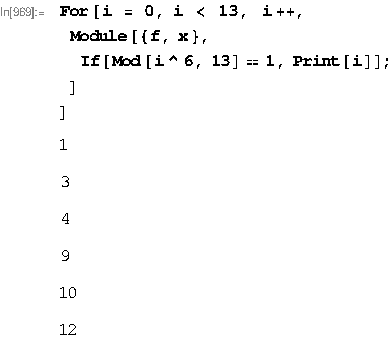
\includegraphics{hw5_1.pdf}
    \caption{Mathematica code prints the 
    solutions to $x^6 \equiv 1 \mod 13$}
    \label{fig:1}
  \end{figure}
\vfill
\clearpage
\newpage



% PROBLEM 2
\phantom{\quad} \vfill
\noindent
\textbf{Problem} (3.2.8) \\[4ex]
\emph{Solution.} \\[2ex]
  We want to find all primes $p$ such that 
  $\left( \frac{10}{p} \right) = 1$.

  From theorem 3.1(2) we have
  \begin{align*}
    \left( \frac{10}{p} \right)  
    &=
      \left( \frac{2}{p} \right)  
      \left( \frac{5}{p} \right).   
  \end{align*}
  From theorem 3.3, we know that
  if $p$ is an odd prime, then
  $\left( \frac{2}{p} \right) = (-1)^{\frac{p^2-1}{8}}$.
  If $p$ is odd, then $p \equiv \pm 1, \pm 3 \mod 8$.
  if $p \equiv \pm 1 \mod 8$, then $\frac{p^2-1}{8}$ is even.
  If $p \equiv \pm 3 \mod 8$, then $\frac{p^2 - 1}{8}$ is odd.
  From this, we see that
  \begin{align*}
    \left( \frac{2}{p} \right)
    =
    \begin{cases}
      \phantom{-} 1 & \text{if $p \equiv \pm 1 \mod 8$} \\
      \phantom{-} 0 & \text{if $p \equiv \phantom{\pm}0 \mod 2$} \\
      -1 & \text{if $p \equiv \pm 3 \mod 8$} 
    \end{cases}
  \end{align*}

  From theorem 3.4, quadratic reciprocity, we know that 
  $\left( \frac{5}{p} \right) = 
   \left( \frac{p}{5} \right)$
   given $5 \equiv 1 \mod 4$.
  By theorem 3.1(1), 
  \begin{align*}
    \left( \frac{p}{5} \right)
    &\equiv
      p^{\frac{5-1}{2}}  \mod 5 \\
    &\equiv
      p^2 \mod 5.
  \end{align*}
  By lemma 2.10, 
  $p^2 \equiv 1 \mod 5$
  only has solutions for
  $p \equiv \pm 1 \mod 5$.
  Thus, 
  \begin{align*}
    \left( \frac{p}{5} \right)
    &=
      \begin{cases}
        \phantom{-} 1 & \text{if $p \equiv \pm 1 \mod 5$} \\
        \phantom{-} 0 & \text{if $p \equiv \phantom{\pm}0 \mod 5$} \\
        -1 & \text{if $p \equiv \pm 2 \mod 5$}
      \end{cases}
  \end{align*}
  
  We see that 
  $\left( \frac{10}{p} \right) = 1$
  when 
  $p \equiv \pm 1 \mod 5$
  and
  $p \equiv \pm 1 \mod 8$
  or
  $p \equiv \pm 2 \mod 5$
  and
  $p \equiv \pm 3 \mod 8$.
  By the Chinese remainder theorem, there will be
  $2 \cdot 2 + 2 \cdot 2 = 8$ solutions.

  To find the solutions, first we solve
  the set of congruences
  \begin{align*}
    p &\equiv \pm 1 \mod 5 \\
    p &\equiv \pm 1 \mod 8.
  \end{align*}
  Clearly, if 
  $p \equiv 1 \mod 5$ 
  and 
  $p \equiv 1 \mod 8$,
  then 
  $p \equiv 1 \mod 40$ is a solution.
  A similar argument can be used to show
  $p \equiv -1 \mod 40$ is a solution.
  To solve the set of congruences
  \begin{align*}
    p &\equiv - 1 \mod 5 \\
    p &\equiv  1 \mod 8,
  \end{align*}
  we start with the second congruence whose solution is
  $1 + 8k$ for $k \in \mathbb{Z}$.
  Plugging this into the first congruence, we see that
  \begin{align*}
    1 + 8 k &\equiv -1 \mod 5 \\
     8 k &\equiv -2 \mod 5 \\
     3 k &\equiv 3 \mod 5 \\
     k &\equiv 1 \mod 5, 
  \end{align*}
  so $k = 1 + 5l$ for $l \in \mathbb{Z}$.
  Now we have our solution
  \begin{align*}
    1 + 8k &= 1 + 8(1 + 5l) \\ 
           &= 9 + 40l.
  \end{align*}
  For a solution $p$,
  we see that
  $p \equiv 9 \mod 40$.

  Now we solve the final congruence
  \begin{align*}
    p &\equiv  1 \mod 5 \\
    p &\equiv - 1 \mod 8,
  \end{align*}
  We start with the solution to the second congruence,
  $-1 + 8k$, $k \in \mathbb{Z}$.
  Plugging this into the first congruence, we see that
  \begin{align*}
    -1 + 8 k &\equiv 1 \mod 5 \\
     8 k &\equiv 2 \mod 5 \\
     3 k &\equiv -3 \mod 5 \\
     k &\equiv -1 \mod 5, 
  \end{align*}
  so $k = -1 + 5l$ for $l \in \mathbb{Z}$.
  Now we have our solution
  \begin{align*}
    -1 + 8k &= -1 + 8(-1 + 5l) \\ 
           &= -9 + 40l \\
           &= 31 + 40l' & l' \in \mathbb{Z}
  \end{align*}
  For a solution $p$,
  we see that
  $p \equiv 31 \mod 40$.

  At this point, our first four solutions are
  $p \equiv \pm 1, \pm 9 \mod 40$. 
  Finding the remaining four involves solving the set
  of congruences
  \begin{align*}
    p &\equiv \pm 2 \mod 5 \\
    p &\equiv \pm 3 \mod 8.
  \end{align*}
  Finding the solutions to these congrunces is equally 
  tedious. 
  Since finding the solutions to the chinese remainder
  theorem is not the point of this exercise, I will 
  list the remaining four solutions:
  $p \equiv \pm 3, \pm 13 \mod 40$.

  Therefore, 
  $\left( \frac{10}{p} \right) = 1$ 
  when
  $p \equiv \pm 1, \pm 3, \pm 9, \pm 13 \mod 40$.
\vfill
\newpage



% PROBLEM 3
\phantom{\quad} \vfill
\noindent
\textbf{Problem} (3.2.18) \\[4ex]
\emph{Solution.} \\[2ex]
  For $q = 1111111111111$, where $q$ is prime, 
  we wish to find whether or not $1001$ is a 
  quadratic residue mod $q$.

  First we note that 
  $111 \cdot 1001 = 111111$.
  Using this, we see that
  \begin{align*}
    q &= 
    \left( 
          111 \cdot 1001 \cdot 10^7 
          +
          111 \cdot 1001 
    \right)
    + 1 \\
    &=
      (111 \cdot 10^7 + 111)1001 + 1.
  \end{align*}
  Since $0 \leq 1 < 1001$, by the division
  algorithm, 1 is the remainder when
  $q$ is divided by 1001.
  Thus, $q \equiv 1 \mod 1001$.
  Since $1001 = 7 \cdot 11 \cdot 13$,
  by theorem 2.3(3), 
  \begin{align}
    \label{eq:3.2.18.1}
    q &\equiv 1 \mod 7 \\
    \label{eq:3.2.18.2}
    q &\equiv 1 \mod 11 \\
    \label{eq:3.2.18.3}
    q &\equiv 1 \mod 13. 
  \end{align}
  
  By theorem 3.1(2), we have
  \begin{align*}
    \left( \frac{1001}{q} \right)
    &=
      \left( \frac{7}{q} \right)
      \left( \frac{11}{q} \right)
      \left( \frac{13}{q} \right).
  \end{align*}

  Using theorem 3.1(3) and 3.4, we see that
  \begin{align*}
    \left( \frac{7}{q} \right)
    &=
    -\left( \frac{q}{7} \right) & \text{since $q \equiv 3 \mod 4$ 
                                        and $7 \equiv 3 \mod 4$}\\
    &=
     -\left( \frac{1}{7} \right) & \text{from equation \ref{eq:3.2.18.1}}\\
    &=
      -1.
  \end{align*}
  Likewise, we see that
  \begin{align*}
    \left( \frac{11}{q} \right)
    &=
    -\left( \frac{q}{11} \right) & \text{since $q \equiv 3 \mod 4$ 
                                        and $11 \equiv 3 \mod 4$}\\
    &=
     -\left( \frac{1}{11} \right) & \text{from equation \ref{eq:3.2.18.2}}\\
    &=
      -1,
  \end{align*}
  and 
  \begin{align*}
    \left( \frac{13}{q} \right)
    &=
      \left( \frac{q}{13} \right) & \text{since $13 \equiv 1 \mod 4$}\\
    &=
      \left( \frac{1}{13} \right) & \text{from equation \ref{eq:3.2.18.3}}\\
    &=
      1
  \end{align*}

  Now we have enough information to determine whether 1001 is
  a quadratic residue modulo $q$.
  We see that
  \begin{align*}
    \left( \frac{1001}{q} \right)
    &=
      \left( \frac{7}{q} \right)
      \left( \frac{11}{q} \right)
      \left( \frac{13}{q} \right). \\
    &=
      -1 \cdot -1 \cdot 1 \\
    &= 
      1.
  \end{align*}
  By definition, 1001 is a quadratic residue modulo $q$.

\vfill
\newpage



% PROBLEM 4
\phantom{\quad} \vfill
\noindent
\textbf{Problem} (3.3.4) \\[4ex]
\emph{Solution.} \\[2ex]
  We want to determine whether 
  the congruence
  $x^4 \equiv 25 \mod 1013$ 
  has solutions given that $1013$ is prime.

  We see that 
  $x^4 = \left( x^2 \right)^2 = 25 \mod 1013$,
  so it is sufficient to prove that
  $x^2 \equiv \pm 5 \mod 1013$ has solutions.

  First we consider $x^2 \equiv 5 \mod 1013$.
  Using theorem 3.4, or quadratic reciprocity, and the
  fact that $5 \equiv 1 \mod 4$, we see that 
  \begin{align*}
    \left( \frac{5}{1013} \right)
    &=
      \left( \frac{1013}{5} \right) \\
    &=
      \left( \frac{3}{5} \right) \\
    &=
      -1,
  \end{align*}
  because by inspection
  \begin{align*}
    \left( \frac{a}{5} \right)
    &=
      \begin{cases}
        \phantom{-}1 & \text{if $a \equiv \pm 1 \mod 5$} \\
        -1 & \text{if $a \equiv \pm 3 \mod 5$} \\
      \end{cases}
  \end{align*}
  By definition, $x^2 \equiv 5 \mod 1013$ has no solutions.

  Second we consider $x^2 \equiv -5 \mod 1013$.
  Using theorem 3.1, we see that
  \begin{align*}
    \left( \frac{-5}{1013} \right)
    &=
      \left( \frac{-1}{1013} \right)
      \left( \frac{5}{1013} \right) \\
    &=
      (-1)^{\frac{1013-1}{2}} \cdot (-1) & \text{(from our earlier work)} \\
    &=
      (-1)^{506} \cdot (-1) \\
    &=
      1 \cdot -1 \\
    &= 
      -1.
  \end{align*}
  By definition, $x^2 \equiv -5 \mod 1013$ has no solutions.

  Since $x^2 \equiv \pm 5 \mod 1013$ has no solutions and 
  $\pm 5 \mod 1013$ are the only solutions to the congruence
  $y^2 \equiv 25 \mod 1013$, 
  we see that
  $\left( x^2 \right)^2 = x^4 \equiv 25 \mod 1013$ 
  can have no solutions.
\vfill
\newpage



% PROBLEM 5
\phantom{\quad} \vfill
\noindent
\textbf{Problem} (3.3.15) \\[4ex]
\emph{Solution.} \\[2ex]
  We aim to show that for any prime $p \geq 7$, there
  is some number $n \in \mathbb{N}$ where
  $1 \leq n \leq 9$ and 
  \begin{equation}
    \label{eq:3.3.15.1}
    \left( \frac{n}{p} \right) 
    = 
    \left( \frac{n+1}{p} \right) 
    = 
    1.
  \end{equation}

  We have three cases
  \begin{enumerate}[1.]
    \item $p \equiv \pm 1 \mod 8$: \\
      Clearly,
      $\left( \frac{1}{p} \right) = 1$.
      By theorem 3.3, 
      $\left( \frac{2}{p} \right) = (-1)^{\frac{p^2-1}{8}}$.
      Clearly, 
      $\left( \frac{2}{p} \right) = 1$ 
      if 
      $\frac{p^2-1}{8}$ is even.
      Since $p \equiv \pm 1 \mod 8$, we may write $p$ as
      $1 + 8k$ for some $k \in \mathbb{Z}$.
      Now we see that
      \begin{align*}
        p &= \pm 1 + 8k \\
        p^2 &= 1 \pm 16k + 64k \\
        p^2 - 1 &= \pm 16k + 64k \\
        \frac{p^2 - 1}{8} &= \pm 2k + 8k \\
        \frac{p^2 - 1}{8} &\equiv 0 \mod 2,
      \end{align*}
      so
      $\left( \frac{1}{p} \right) = 1$
      and 
      $\left( \frac{2}{p} \right) = 1$.
      Therefore, equation \ref{eq:3.3.15.1} is true for $n = 1$.
    \item $p \equiv \pm 1 \mod 5$:  \\
      Clearly, 
      $\left( \frac{4}{p} \right) = 1$.
      By theorem 3.4, or quadratic reciprocity,
      $\left( \frac{5}{p} \right) = \left( \frac{p}{5} \right)$.
      By inspection, the only quadratic residues modulo 5
      are the congruence classes $\pm 1$.
      By assumption, $p \equiv \pm 1 \mod 5$, so 
      $\left( \frac{5}{p} \right) = 1$. 
      Therefore, equation \ref{eq:3.3.15.1} is true for $n = 4$.
    \item $p \equiv \pm 2 \mod 5$ and $p \equiv \pm 3 \mod 8$: \\
      Clearly, 
      $\left( \frac{9}{p} \right) = 1$.
      Our earlier work in problem 3.2.8 shows us that
      $\left( \frac{10}{p} \right) = 1$
      when $p \equiv \pm 2 \mod 5$ and $p \equiv \pm 3 \mod 8$.
      This is true by assumption, so equation 
      \ref{eq:3.3.15.1} is true for $n = 9$.
  \end{enumerate}
  Since $p \geq 7$, we see that $p$ is odd.
  We have covered all cases because $p$ must be congruent to one of
  $\pm 1, \pm 3 \mod 8$ and congruent to one of 
  $\pm 1, \pm 2 \mod 5$.
  Therefore, equation \ref{eq:3.3.15.1} is true for some 
  $n \in \mathbb{Z}$ 
  where
  $1 \leq n \leq 9$.
\vfill
\newpage



% PROBLEM 6
\phantom{\quad} \vfill
\noindent
\textbf{Problem} (3.4.1) \\[4ex]
\emph{Solution.} \\[2ex]
	\begin{enumerate}
		\item[a.]
      For the binary quadratic form
      \[
        f(x,y) = x^2 + y^2,
      \]
      we have
      \begin{align*}
        d &= b^2 - 4ac \\
          &= 0^2 - 4 (1)(1) \\
          &= -4 \\
          &< 0,
      \end{align*}
      so given that $a$ and $c$
      have the same sign and $a > 0$, 
      by theorem 3.11, $f(x,y)$ is 
      \textbf{positive definite}.
		\item[b.]
      For the binary quadratic form
      \[
        f(x,y) = -x^2 - y^2,
      \]
      Since $x^2 + y^2$ is positive definite
      and $f(x,y) = -(x^2 + y^2)$, 
      clearly $f(x,y)$ is \textbf{negative definite}.
		\item[c.]
     For the binary quadratic form
      \[
        f(x,y) = x^2 - 2y^2,
      \]
      we have
      \begin{align*}
        d &= b^2 - 4ac \\
          &= 0^2 - 4 (1)(-2) \\
          &= 8 \\
          &> 0,
      \end{align*}
      so by theorem 3.11, 
      $f(x,y)$ is \textbf{indefinite.}
		\item[d.]
     For the binary quadratic form
      \[
        f(x,y) = 10x^2 - 9xy + 8y^2
      \]
      we have
      \begin{align*}
        d &= b^2 - 4ac \\
          &= (-9)^2 - 4(10)(8) \\
          &= 81 - 320 \\
          &= -239 \\
          &< 0.
      \end{align*}
      We see that $a = 10$, $c = 8$ have the same sign
      and that $a > 0$,
      so by theorem 3.11, 
      $f(x,y)$ is \textbf{positive definite}.
		\item[e.]
     For the binary quadratic form
      \[
        f(x,y) = x^2 - 3xy + y^2
      \]
      we have
      \begin{align*}
        d &= b^2 - 4ac \\
          &= (-3)^2 - 4(1)(1) \\
          &= 9 - 4 \\
          &= 5 \\
          &> 0,
      \end{align*}
      so by theorem 3.11, 
      $f(x,y)$ is \textbf{indefinite}.
		\item[f.]
      For the binary quadratic form
      \[
        f(x,y) = 17x^2 - 26xy + 10y^2
      \]
      we have
      \begin{align*}
        d &= b^2 - 4ac \\
          &= (-26)^2  - 4(17)(10) \\
          &= 576 - 680 \\
          &= -104 \\
          &< 0.
      \end{align*}
      We see that $a = 17$ and $c = 10$ have the 
      same sign and that $a > 0$, 
      so by theorem 3.11, 
      $f(x,y)$ is \textbf{positive definite}.
	\end{enumerate}
\vfill
\newpage



% PROBLEM 7
\phantom{\quad} \vfill
\noindent
\textbf{Problem} (3.3.4) \\[4ex]
\emph{Solution.} \\[2ex]
  First we find a formula for positive integers
  $x_k$ and $y_k$ such that 
  $(3 + 2 \sqrt{2})^k = x_k + \sqrt{2}y_k$.

  We see that 
  \begin{align*}
    (3 + 2 \sqrt{2})^k 
    &=
      \sum_{\substack{i = 0}}^k
        \binom{k}{i}
        3^{k-i}
        (2\sqrt{2})^i \\
    &=
        \sum_{\substack{i = 0 \\ \text{$i$ even}}}^k
        \binom{k}{i}
        3^{k-i}
        (2\sqrt{2})^i 
        +
        \sum_{\substack{j = 0 \\ \text{$j$ odd}}}^k
        \binom{k}{j}
        3^{k-j}
        (2\sqrt{2})^j \\
    &=
        \sum_{\substack{i = 0 \\ \text{$i$ even}}}^k
        \binom{k}{i}
        3^{k-i}
        \cdot
        2^i 
        \cdot
        2^{i/2} 
        +
        \sum_{\substack{j = 0 \\ \text{$j$ odd}}}^k
        \binom{k}{j}
        3^{k-j}
        \cdot
        2^j 
        \cdot
        (\sqrt{2})^{j-1} 
        \cdot
        \sqrt{2} \\
    &=
        \sum_{\substack{i = 0 \\ \text{$i$ even}}}^k
        \binom{k}{i}
        3^{k-i}
        \cdot
        2^{\frac{3i}{2}}
        +
        \sqrt{2}
        \sum_{\substack{j = 0 \\ \text{$j$ odd}}}^k
        \binom{k}{j}
        3^{k-j}
        \cdot
        2^{\frac{3j-1}{2}}.
  \end{align*}
  Thus, such a representation is possible for 
  \begin{align*}
    x_k
    &=
      \sum_{\substack{i = 0 \\ \text{$i$ even}}}^k
        \binom{k}{i}
        3^{k-i}
        \cdot
        2^{\frac{3i}{2}} \\
    y_k 
    &=
        \sum_{\substack{j = 0 \\ \text{$j$ odd}}}^k
        \binom{k}{j}
        3^{k-j}
        \cdot
        2^{\frac{3j-1}{2}}.
  \end{align*}

  Next we show that $(3 - 2\sqrt{2})^k = x_k - y_k$.
  \begin{align*}
    (3 - 2 \sqrt{2})^k 
    &=
      \sum_{\substack{i = 0}}^k
        \binom{k}{i}
        3^{k-i}
        (-2\sqrt{2})^i \\
    &=
        \sum_{\substack{i = 0 \\ \text{$i$ even}}}^k
        \binom{k}{i}
        3^{k-i}
        (-2\sqrt{2})^i 
        +
        \sum_{\substack{j = 0 \\ \text{$j$ odd}}}^k
        \binom{k}{j}
        3^{k-j}
        (-2\sqrt{2})^j \\
    &=
        \sum_{\substack{i = 0 \\ \text{$i$ even}}}^k
        \binom{k}{i}
        3^{k-i}
        (2\sqrt{2})^i
        \cdot (-1)^i
        +
        \sum_{\substack{j = 0 \\ \text{$j$ odd}}}^k
        \binom{k}{j}
        3^{k-j}
        (2\sqrt{2})^j 
        \cdot
        (-1)^j
        \\
    &=
        \sum_{\substack{i = 0 \\ \text{$i$ even}}}^k
        \binom{k}{i}
        3^{k-i}
        (2\sqrt{2})^i
        -
        \sum_{\substack{j = 0 \\ \text{$j$ odd}}}^k
        \binom{k}{j}
        3^{k-j}
        (2\sqrt{2})^j \\
    &=
        \sum_{\substack{i = 0 \\ \text{$i$ even}}}^k
        \binom{k}{i}
        3^{k-i}
        \cdot
        2^i 
        \cdot
        2^{i/2} 
        -
        \sum_{\substack{j = 0 \\ \text{$j$ odd}}}^k
        \binom{k}{j}
        3^{k-j}
        \cdot
        2^j 
        \cdot
        (\sqrt{2})^{j-1} 
        \cdot
        \sqrt{2} \\
    &=
        \sum_{\substack{i = 0 \\ \text{$i$ even}}}^k
        \binom{k}{i}
        3^{k-i}
        \cdot
        2^{\frac{3i}{2}}
        -
        \sqrt{2}
        \sum_{\substack{j = 0 \\ \text{$j$ odd}}}^k
        \binom{k}{j}
        3^{k-j}
        \cdot
        2^{\frac{3j-1}{2}} \\
    &=
        x_k - \sqrt{2} y_k
  \end{align*}

  Now we deduce that $x_k^2 - 2y_k^2 = 1$ for 
  $k = 1,2,3. \ldots$. 

  We see that 
  \begin{align*}
    x_k^2 - 2y_k^2
    &=
      (x_k + \sqrt{2}y_k)
      (x_k - \sqrt{2}y_k) \\
    &=
      (3 + 2 \sqrt{2})^k
      (3 - 2 \sqrt{2})^k \\
    &=
      \left[
        (3 + 2 \sqrt{2})
        (3 - 2 \sqrt{2})
      \right]^k \\
    &=
      (9 - 4 \cdot 2)^k  \\
    &=
      (9 - 8)^k \\
    &=
      1^k \\
    &=
      1\ \text{for all $k = 1,2,3,\ldots$}
  \end{align*}

  Now we show $\gcd(x_k, y_k) = 1$.
  By theorem 1.3, the greatest common divisor 
  or $x_k^2$ and $y_k^2$ is the smallest positive
  integer that is a linear combination of the two
  with integer coefficients.
  Since we have showed that 
  $x_k^2 - 2y_k = 1$, 
  we see that $\gcd(x_k^2, y_k^2) = 1$
  because there are no positive integers smaller than 1.
  By definition, two coprime numbers share no 
  prime factors.
  Since the prime factors of $x_k$ are a subset of 
  $x_k^2$ and the prime factors of $y_k$ are a subset
  of $y_k^2$, we see that
  $x_k, y_k$ cannot share any prime factors. 
  Thus, they are coprime and 
  $\gcd(x_k, y_k) = 1$ for all $k \in \mathbb{N}$.

  Next we show that 
  $x_{k+1} = 3x_k + 4y_k$
  and 
  $y_{k+1} = 2x_k + 3y_k$
  for all $k \in \mathbb{N}$.
  We see that 
  \begin{align*}
    x_k
    &=
      \sum_{\substack{i = 0 \\ \text{$i$ even}}}^k
        \binom{k}{i}
        3^{k-i}
        \cdot
        2^{\frac{3i}{2}} \\
    x_{k+1}
    &=
      \sum_{\substack{i = 0 \\ \text{$i$ even}}}^{k+1}
        \binom{k+1}{i}
        3^{k+1-i}
        \cdot
        2^{\frac{3i}{2}} \\
    y_k 
    &=
        \sum_{\substack{j = 0 \\ \text{$j$ odd}}}^k
        \binom{k}{j}
        3^{k-j}
        \cdot
        2^{\frac{3j-1}{2}} \\
    y_{k+1}
    &=
      \sum_{\substack{j = 0 \\ \text{$j$ odd}}}^{k+1}
        \binom{k+1}{j}
        3^{k+1-j}
        \cdot
        2^{\frac{3j-1}{2}}.
  \end{align*}
  We see that 
  \begin{align*}
    3x_k + 4y_k 
    &=
      3
      \sum_{\substack{i = 0 \\ \text{$i$ even}}}^k
        \binom{k}{i}
        3^{k-i}
        \cdot
        2^{\frac{3i}{2}}
      +
      4
      \sum_{\substack{j = 0 \\ \text{$j$ odd}}}^k
        \binom{k}{j}
        3^{k-j}
        \cdot
        2^{\frac{3j-1}{2}} \\
    &=
      \sum_{\substack{i = 0 \\ \text{$i$ even}}}^k
        \binom{k}{i}
        3^{k+1-i}
        \cdot
        2^{\frac{3i}{2}}
      +
      \sum_{\substack{j = 0 \\ \text{$j$ odd}}}^k
        \binom{k}{j}
        3^{k-j}
        \cdot
        2^{\frac{3j+3}{2}} \\
    &=
      \sum_{\substack{i = 0 \\ \text{$i$ even}}}^{k+1}
        \binom{k}{i}
        3^{k+1-i}
        \cdot
        2^{\frac{3i}{2}}
      +
      \sum_{\substack{j = 0 \\ \text{$j$ even}}}^{k+1}
        \binom{k}{j-1}
        3^{k-(j-1)}
        \cdot
        2^{\frac{3(j-1)+3}{2}} \\
    &=
        \sum_{\substack{i = 0 \\ \text{$i$ even}}}^{k+1}
        \binom{k}{i}
        3^{k+1-i}
        \cdot
        2^{\frac{3i}{2}}
        + 
        \binom{k}{i-1}
        3^{k-(i-1)}
        \cdot
        2^{\frac{3(i-1)+3}{2}} \\
    &=
        \sum_{\substack{i = 0 \\ \text{$i$ even}}}^{k+1}
        \left[
          \binom{k}{i}
          +
          \binom{k}{i-1}
        \right]
        3^{k+1-i}
        \cdot
        2^{\frac{3i}{2}} \\
    &=
        \sum_{\substack{i = 0 \\ \text{$i$ even}}}^{k+1}
        \binom{k+1}{i}
        3^{k+1-i}
        \cdot
        2^{\frac{3i}{2}} \\
    &=
        x_{k+1},
  \end{align*}
  where we have made use of the equality
  \[
    \binom{n}{k} = \binom{n}{n-k},
  \]
  as outlined in equation 1.10 of Zuckerman et al.

  Likewise, we see that
  \begin{align*}
    2x_k + 3y_k
    &=
      2
      \sum_{\substack{i = 0 \\ \text{$i$ even}}}^k
        \binom{k}{i}
        3^{k-i}
        \cdot
        2^{\frac{3i}{2}}
      +
      3
      \sum_{\substack{j = 0 \\ \text{$j$ odd}}}^k
        \binom{k}{j}
        3^{k-j}
        \cdot
        2^{\frac{3j-1}{2}} \\
    &=
      \sum_{\substack{i = 0 \\ \text{$i$ even}}}^k
        \binom{k}{i}
        3^{k-i}
        \cdot
        2^{\frac{3i+2}{2}}
      +
      \sum_{\substack{j = 0 \\ \text{$j$ odd}}}^k
        \binom{k}{j}
        3^{k+1-j}
        \cdot
        2^{\frac{3j-1}{2}} \\
    &=
        \sum_{\substack{i = 0 \\ \text{$i$ odd}}}^{k+1}
        \binom{k}{i-1}
        3^{k-(i-1)}
        \cdot
        2^{\frac{3(i-1)+2}{2}}
      +
      \sum_{\substack{j = 0 \\ \text{$j$ odd}}}^k
        \binom{k}{j}
        3^{k+1-j}
        \cdot
        2^{\frac{3j-1}{2}} \\
    &=
      \sum_{\substack{j = 0 \\ \text{$j$ odd}}}^{k+1}
      \left[
        \binom{k}{j}
        + 
        \binom{k}{j-1}
      \right]
      3^{k+1-j}
      2^{\frac{3j-1}{2}} \\
    &=
      \sum_{\substack{j = 0 \\ \text{$j$ odd}}}^{k+1}
      \binom{k+1}{j}
      3^{k+1-j}
      \cdot
      2^{\frac{3j-1}{2}} \\
    &=
      y_{k+1}
  \end{align*}

  Next we show that $\{x_k\}$ and $\{y_k\}$ are
  strictly increasing
  sequences.

  For $i,k \in \mathbb{N}$, we see that
  \begin{align*}
    -i &< 2k + 2 \\
    -i + (k + 1) &< 2k+1 + (k + 1) \\
    k - i + 1 &< 3k + 3 \\
    \frac{(k)(k-1)(k-2)\cdots(k-i+2)}{(i)!} (k-i+1)
      &< 3(k+1)\frac{(k)(k-1)(k-2)\cdots(k-i+2)}{(i)!} \\
    \frac{(k)(k-1)(k-2)\cdots(k-i+2)(k-i+1)}{(i)!}
      &< 3\frac{(k+1)(k)(k-1)(k-2)\cdots(k-i+2)}{(i)!} \\
    \binom{k}{i}
      &< 3\binom{k+1}{i} \\
    3^{k-i}\binom{k}{i}
      &< 3^{k-i} \cdot 3 \cdot \binom{k+1}{i} \\
    \binom{k}{i}\cdot 3^{k-i}
      &< \binom{k+1}{i}\cdot 3^{k+1-i}.
  \end{align*}
  Suppose $i$ is even.
  From this we see that 
  \begin{align*}
    \binom{k}{i}\cdot 3^{k-i}
      &< \binom{k+1}{i}\cdot 3^{k+1-i} \\
    \binom{k}{i}\cdot 3^{k-i} \cdot 2^{\frac{3i}{2}}
      &< \binom{k+1}{i}\cdot 3^{k+1-i} \cdot 2^{\frac{3i}{2}} \\
    x_k &< x_{k+1}.
  \end{align*}
  It is easy to see that for $m < n$, $x_m < x_n$.
  Thus, $\{x_k\}$ is a monotonic strictly increasing sequence.

  Suppose $i$ is odd.
  From this we see that 
  \begin{align*}
    \binom{k}{i}\cdot 3^{k-i}
      &< \binom{k+1}{i}\cdot 3^{k+1-i} \\
    \binom{k}{i}\cdot 3^{k-i} \cdot 2^{\frac{3i+1}{2}}
      &< \binom{k+1}{i}\cdot 3^{k+1-i} \cdot 2^{\frac{3i+1}{2}} \\
    y_k &< y_{k+1}.
  \end{align*}
  It is easy to see that for $m < n$, $y_m < y_n$.
  Thus, $\{y_k\}$ is a monotonic strictly increasing sequence.

  Finally we show that 1 has infinitely many proper
  representations by the quadratic form $x^2 - 2y^2$.

  We have showed that $x^2_k - 2y^2_k = 1$ for 
  $k \in \mathbb{N}$.
  Furthermore, we showed $\gcd(x_k, y_k) = 1$ for 
  $k \in \mathbb{N}$.
  Lastly, we showed that
  $x_m \neq x_n$ for $m \neq n$ because $m < n$ implies $x_m < x_n$.
  Likewise, we showed that
  $y_m \neq y_n$ for $m \neq n$ because $m < n$ implies $y_m < y_n$.
  From this, we can conclude that there is an infinite 
  sequence $\{(x_k, y_k)\}$ whose distinct members properly
  represent 1. 
\vfill
\newpage



% PROBLEM 8
\phantom{\quad} \vfill
\noindent
\textbf{Problem} (3.3.10) \\[4ex]
\emph{Solution.} \\[2ex]
  We want to show that for
  $f(x,y) = ax^2 + bxy + cy^2$, 
  a quadratic form with integral coefficients,
  that there exist integers
  $x_0, y_0$ not both 0 such that 
  $f(x_0, y_0) = 0$,
  if and only if the discriminant $d$ of $f(x,y)$
  is a perfect square, possibly 0. \\

  \noindent
  $\longrightarrow$ \\
  Suppose there exist two integers, 
  $x_0$ and $y_0$, not both 0, such that
  $f(x_0, y_0) = 0$.
  We know that 
  \[
    4af(x_0, y_0) =  (2ax_0 + by_0)^2 - dy^2_0 = 0.
  \]
  Call $v = 2ax_0 + by_0$.
  We see that 
  \begin{align*}
    v^2 &= dy_0^2 \\
    \frac{v^2}{y_0^2} &= d & \text{for $y_0 \neq 0$} \\
    \left( \frac{v}{y_0} \right)^2 &= d.
  \end{align*}
  Thus, if $y_0 \neq 0$, then $d$ is a perfect square.
  If $y_0 = 0$, then
  $f(x_0, 0) = ax_0^2 = 0$, so $a = 0$.
  Given that $d = b^2 - 4ac$, if $a = 0$ then
  $d = b^2$, so again $d$ is a perfect square. \\

  \noindent
  $\longleftarrow$ \\
  Suppose $d$ is a perfect square.
  Let $d = e^2$ for some $e \in \mathbb{Z}$.
  Given 
  \[
    4af(x_0, y_0) =  (2ax_0 + by_0)^2 - dy_0,
  \]
  we see that 
  \begin{align*}
    (2ax_0 + by_0)^2 - dy^2_0 
      &= (2ax_0 + by_0)^2 - e^2y^2_0 \\
      &= (2ax_0 + by_0 + ey_0)(2ax_0 + by_0 - ey_0) \\
      &= (2ax_0 + (b+e)y_0)(2ax_0 + (b-e)y_0). 
  \end{align*}
  We see that 
  $x_0 = (b-e)$, $y_0 = -2a$ 
  and
  $x_0 = (b+e)$, $y_0 = -2a$ 
  are two solutions.
  If $x_0$ and $y_0$ are not both 0, we are done, so we suppose
  that they are both 0.
  Then $-2a = 0$ implies $a = 0$ and 
  $b-e = 0$ and $b + e = 0$ imply $b = e = 0$.
  Plugging in $a = b = 0$, we see that
  $f(x,y) = cy^2$.
  Clearly, $x_0 = 1$, $y_0 = 0$ is a solution to
  $f(x,y) = 0$, and they are not both zero.
  Thus if $d$ is a perfect square, there exist integers
  $x_0, y_0$ not both 0, such that $f(x_0, y_0) = 0$.
  \qed
\vfill
\newpage



% PROBLEM 9
\phantom{\quad} \vfill
\noindent
\textbf{Problem} (3.5.1) \\[4ex]
\emph{Solution.} \\[2ex]
  We want to find a reduced form equivalent to the form
  \[
    f(x,y) = 7x^2 + 25 xy + 23y^2.
  \]
  We see that in the original form, 
  $a = 7$, $b = 25$, and $c = 23$.
  We see that $25 = b \not \leq |a| = 7$, so 
  we first apply the matrix
  \[
    \begin{bmatrix} 1 & -2 \\ 0 & 1 \end{bmatrix}.
  \]
  From equations 3.7a-c, we get the new form
  \[
    A_1x^2 + B_1xy + C_1y^2,
  \]
  where 
  \begin{align*}
    A_1 &= f(1,0) = a  \\
      &= 7\\
    B_1 &= 2am_{12} + b \\
      &= 2\cdot 7 \cdot -2 + 25 \\
      &= -28 + 25 \\
      &= -3 \\
    C_1 &= am_{12}^2 + bm_{12} + c \\
      &= 7 \cdot (-2)^2 + 25 \cdot (-2) + 25 \\
      &= 7 \cdot 4 - 50 + 23 \\
      &= 28 - 50 + 23 \\
      &= 1
  \end{align*}
  Now we have 
  \[
    f_1(x,y) = 7x^2 - 3xy + y^2,
  \]
  where $f \sim f_1$.

  We see that $|A_1| \not< |C_1|$ so we apply the matrix
  \[
    \begin{bmatrix}0 & 1 \\ 1 & 0 \end{bmatrix}.
  \]
  From equations 3.7a-c, we get the new form
  \[
    A_2x^2 + B_2xy + C_2y^2,
  \]
  where 
  \begin{align*}
    A_2 &= C_1 \\
      &= 1\\
    B_2 &= -B_1 \\
      &= -(-3) \\
      &= 3 \\
    C_2 &= A_1 \\
      &= 7
  \end{align*}
  Now we have 
  \[
    f_2(x,y) = x^2 + 3xy + 7y^2,
  \]
  where $f_2 \sim f_1$.

  Again, we see that $B_2 \not \leq |A_2|$, so we apply the matrix
  \[
    \begin{bmatrix} 1 & -1 \\ 0 & 1 \end{bmatrix}
  \]
  to get
  \begin{align*}
    A_3 &= f(1,0) = a  \\
      &= 1\\
    B_3 &= 2am_{12} + b \\
      &= 2\cdot 1 \cdot -1 + 3 \\
      &= -2 + 3 \\
      &= 1 \\
    C_3 &= am_{12}^2 + bm_{12} + c \\
      &= 1 \cdot (-1)^2 + 3 \cdot (-1) + 7 \\
      &= 1 - 3 + 7 \\
      &= 5
  \end{align*}
  Now we have 
  \[
    f_3(x,y) = x^2 + xy + 5y^2,
  \]
  where $f_3 \sim f_2$, and $f_3$ is in reduced form.

  By transitivity, $f_3 \sim f$.



\vfill
\newpage



% PROBLEM 10
\phantom{\quad} \vfill
\noindent
\textbf{Problem} (3.5.3) \\[4ex]
\emph{Solution.} \\[2ex]
  For $x,y \in \mathbb{Z}$, we want to show that 
  there exist $u,v \in \mathbb{Z}$ such that
  $
  \begin{bmatrix}
    x & y \\ u & v 
  \end{bmatrix}
  \in \Gamma
  $
  if and only if 
  $\gcd(x,y) = 1$.

  By theorem 1.3, 
  $\gcd(x,y) = 1$ if and only if we can 
  write
  \[
    xv + yu' = 1,
  \]
  for some $u',v \in \mathbb{Z}$.
  Let $u = -u'$. 
  We have
  \[
    xv - yu = 1.
  \]
  Consider the matrix
  \[
    M = 
    \begin{bmatrix}
      x & y \\
      u & v
    \end{bmatrix}.
  \]
  We see that $M \in \Gamma$
  if and only if $\gcd(x,y) = 1$
  because
  $m_{ij} \in \mathbb{Z}$ and
  det $M = xv - yu = 1$ if and only if
  $\gcd(x,y) = 1$.
  \qed

\vfill
\newpage



% PROBLEM 11
\phantom{\quad} \vfill
\noindent
\textbf{Problem} (3.5.11) \\[4ex]
\emph{Solution.} \\[2ex]
  Suppose that $ax^2 + bxy + cy^2 \sim Ax^2 + Bxy + Cy^2$.
  We want to show that $\gcd(a,b,c) = \gcd(A,B,C)$.

  Let $f(x,y) = ax^2 + bxy + cy^2$ and 
  $h(x,y) = Ax^2 + Bxy + Cy^2$.
  Since $f \sim h$, they represent the same points.
  Let $g = \gcd(a,b,c)$ and $G = \gcd(A,B,C)$.
  Clearly, $\frac{f(x,y)}{g} \in \mathbb{Z}$.
  Because $f$ and $h$ represent the same points, 
  $\frac{h(x,y)}{g} \in \mathbb{Z}$ as well.
  We see that $h(1,0) = A$ and $h(0,1) = C$, 
  so $g \mid A$ and $g \mid C$. 
  Again, $h(1,1) = A + B + C$ and because
  $g \mid h(x,y)$, then $g \mid B$ as well.
  So $g$ is a common divisor of $A$,$B$, and $C$.
  Thus, $g \mid G$.

  Likewise, $G \mid h(x,y)$ 
  $G \mid f(x,y)$ for all $x,y \in \mathbb{Z}$.
  We see that 
  $f(1,0) = a$ 
  and 
  $f(0,1) = c$, 
  so 
  $G \mid a$ and $G \mid c$. 
  Again, $f(1,1) = a + b + c$ and because
  $G \mid f(x,y)$, then $G \mid b$ as well.
  So $G$ is a common divisor of $a$,$b$, and $c$.
  Thus, $G \mid g$.

  Since $g \mid G$ and $G \mid g$, 
  $g = \pm G$.
  But the greatest common divisor is always positive, 
  so $g = G$.
\vfill
\newpage



% PROBLEM 12
\phantom{\quad} \vfill
\noindent
\textbf{Problem} (3.5.12) \\[4ex]
\emph{Solution.} \\[2ex]
  Suppose $f(x,y) = ax^2 + bxy + cy^2$ is a positive
  semidefinite quadratic form of discriminant 0.
  Let $g = \gcd(a,b,c)$. 
  We want to show that $f$ is equivalent to the form $gx^2$.

  We see that $d = b^2 - 4ac = 0$, so 
  \begin{equation}
    \label{eq:3.5.12.1}
    ac = \left( \frac{b}{2} \right)^2,
  \end{equation}
  So the product $ac$ is a square.
  Consider the prime factorization of 
  $a$ and $c$ such that 
  \begin{align*}
    a &= \prod_{p} p^{\alpha(p)} \\
    c &= \prod_{p} p^{\gamma(p)},
  \end{align*}
  for primes $p$.
  Clearly, 
  \begin{equation}
    \label{eq:3.5.12.2}
    \alpha(p) + \gamma(p) \equiv 0 \mod 2.
  \end{equation}
  Let $g = \gcd(a,b,c)$ be factored as
  \[
    g = \prod_p p^{\text{min}(\alpha(p),\beta(p), \gamma(p))}. 
  \]
  Considering equation \ref{eq:3.5.12.1}, we see that
  $\text{min}(\alpha(p),\beta(p), \gamma(p)) = 
  \text{min}\left(\alpha(p),
                  \frac{\alpha(p) + \gamma(p)}{2}, \gamma(p)\right)$,
  if $p \neq 2$ and 
  $\text{min}\left(\alpha(2),
                  \frac{\alpha(2) + \gamma(2) + 1}{2}, \gamma(2)\right)$,
  if $p = 2$.
  Furthermore, we see that if 
  $\alpha(p) \leq \gamma(p)$, then 
  \begin{align*}
    \alpha(p) &= \frac{2\alpha(p)}{2} \\
              &= \frac{\alpha(p) + \alpha(p)}{2} \\
              &\leq \frac{\gamma(p) + \alpha(p)}{2},
  \end{align*}
  and if 
  $\gamma(p) \leq \alpha(p)$, then 
  \begin{align*}
    \gamma(p) &= \frac{2\gamma(p)}{2} \\
              &= \frac{\gamma(p) + \gamma(p)}{2} \\
              &\leq \frac{\gamma(p) + \alpha(p)}{2}.
  \end{align*}
  Therefore, 
  the exponents of the greatest common divisor in its
  prime factorization have the form
  $\text{min}(\alpha(p), \gamma(p))$.

  By definition of a divisor, 
  there is some $n \in \mathbb{Z}$ such that
  $ng = a$.
  Consider the prime factorization of $n$.
  We see that 
  \[
    n = 2^j \prod_{p\neq 2} p^{\alpha(p) - 
                 \text{min}\left(\alpha(p),
                            \gamma(p)\right)
                 },
  \]
  for some $j \in \mathbb{N}$.
  From equation \ref{eq:3.5.12.2}, we see that 
  $\alpha(p)$ and $\gamma(p)$ have the same parity.
  That is, they are both even or both odd. 

  Thus, we see that 
  $\alpha(p) - \text{min}(\alpha(p), \gamma(p))$
  is even, so $n$ is a perfect square. 
  Let $m^2 = n$ for some $m \in \mathbb{Z}$.
  We see that 
  \begin{align*}
    4af(x,y) &= (2ax + by)^2 - dy^2 \\
    4af(x,y) &= (2ax + by)^2 \\
    f(x,y) &= \frac{(2ax + by)^2}{4a} \\
    f(x,y) &= \frac{g^2\left( \frac{2ax}{g} + \frac{by}{g} \right)^2}{4ng} \\
    f(x,y) &= \frac{g\left( \frac{2ax}{g} + \frac{by}{g} \right)^2}{4n} \\
    f(x,y) &= \frac{g\left( \frac{2ax}{g} + \frac{by}{g} \right)^2}{4m^2} \\
    f(x,y) &= g\left( \frac{2ax + by}{2mg} \right)^2,
  \end{align*}
  so all values of $f(x,y)$ can be represented by $gx^2$. 

  Call $h(x,y) = gx^2$. 
  We see that
  \begin{align*}
    f(x,y) = g\left(\frac{2a}{2mg}x + \frac{b}{2mg}y, ux + vy\right),
  \end{align*}
  where $u$ and $v$ are such that 
  \[
    \frac{a}{mg} v - \frac{b}{2mg}u = 1.
  \]
  Such numbers $u,v$ will exist if
  $\gcd\left( \frac{a}{mg}, \frac{b}{2mg}\right) = 1$.
  We also see that $\frac{a}{mg} = m$ because 
  $a = ng = m^2 g$. 

  We aim to show that $\gcd \left(m, \frac{b}{2mg} \right) = 1$.
  We see that $ac = m^2 g c = \left( \frac{b}{2} \right)^2$,
  so $m^2 \mid (b^2/4)$, so $m \mid (b/2)$.

  Now we note that if $\gcd(a,b,c) = g$, then
  $\gcd\left(\frac{a}{g}, \frac{b}{g}, \frac{c}{g} \right) = 1$.
  We see that 
  \begin{align*}
    ac &= \left( \frac{b}{2} \right)^2 \\
    c &= \frac{1}{a} \left( \frac{b}{2} \right)^2 \\ 
    c &= \frac{1}{m^2 g} \left( \frac{b}{2} \right)^2 \\ 
    c &= \frac{1}{m^2 g}\cdot \frac{b}{2} \cdot \frac{b}{2} \\
    \frac{c}{g} &= \cdot \frac{b}{2mg} \cdot \frac{b}{2mg}.
  \end{align*}
  Also, 
  \begin{align*}
    \frac{a}{g} &= \frac{m^2 g}{g} \\
                &= m^2.
  \end{align*}
  So 
  \[
    \gcd \left( m^2, \frac{b}{g}, \frac{b}{2mg} \cdot \frac{b}{2mg} \right)
      = 1.
  \]
  Clearly, $\gcd\left(m^2, \left(\frac{b}{2mg}\right)^2\right) = 1$
  so we can conclude that 
  $\gcd\left(m, \frac{b}{2mg}\right) = 1$ considering their 
  prime factorizations.

  Therefore, there will be $u,v$ which satisfy 
  \[
    \frac{a}{mg} v - \frac{b}{2mg}u = 1,
  \]
  and the matrix
  \[
    \begin{bmatrix}
      m & \frac{b}{2mg} \\
      u & v
    \end{bmatrix}
    \in \Gamma
  \]
  defines the transformation from $h$ to $f$.
  By definition, $h \sim f$.
\vfill



\end{document}
